\documentclass{uni_tue_template}

\usepackage{color}
\usepackage[colorlinks]{hyperref}
\definecolor{darkred}{rgb}{0.5,0,0}
\definecolor{darkgreen}{rgb}{0,0.5,0}
\definecolor{darkblue}{rgb}{0,0,0.7}
\hypersetup{
			linkcolor={darkblue},
			filecolor={darkgreen},
			urlcolor={darkred},
			citecolor={darkblue},
}

\usepackage[export]{adjustbox}
\usepackage{pgf}
\usepackage{tikz}
\usetikzlibrary{arrows}
\tikzset{<->,>=stealth',shorten >=1pt,auto,node distance=4.5cm,bend angle=20,
		 every path/.style={font=\ttfamily\scriptsize\bfseries},
		 relation/.style={
		 	circle,fill=blue!20,draw,font=\ttfamily\footnotesize\bfseries,
			prefix after command= {\pgfextra{\tikzset{every label/.style={font=\ttfamily\footnotesize\bfseries,yshift=-1cm}}}}
			 }
}
\usepackage{sistyle}

\lstdefinestyle{sql}{%
	language=SQL,%
	commentstyle=\color{comment},%
	stringstyle=\color{string},%
	keywordstyle=\color{keyword}\bfseries,%
	morekeywords={text, real, begin},%
	basicstyle=\ttfamily\footnotesize,%
	numbers=left,
	numberstyle=\tiny\color{black},
	stepnumber=1,
	showstringspaces=true,%
	columns=fixed,%
	moredelim=[is][\itshape]{@@}{@@},%
	tabsize=2
}
\lstset{aboveskip=-.05cm,style=sql, firstline=4}

\newcommand{\otext}[1]{\overset{\mathclap{\rule[-.3\baselineskip]{0pt}{0cm}\textmd{#1}}}}
\newcommand{\set}[1]{\mathbb{#1}}
\newcommand{\code}[1]{\texttt{{\footnotesize #1}}}
\newcommand{\md}[1]{\textmd{#1}}

% content of left head area e.g. subject like ETI
\def \headLeft{Andreas Schmied (3087156),\newline Tobias Stumpp (3798377)}

% content of center head area, used for names
\def \names{\"Ubungsblatt 5,\\ Datenbanksysteme II}

% content of right head area e.g. semester like WiSe 2012/13
\def \headRight{\today}

% set name for exercises
\def \exerciseName{Aufgabe}

\begin{document}
\exercise{}
\subExBegin{1{.}}
  \item \emph{Identifizieren Sie 4 Blattknoten-Einträge $(a,\ldots,d)$, so dass durch sukzessives Einfügen der Werte (\code{insert(a),\ldots,insert(d)}) die Blattebene komplett gefüllt wird.}
  \begin{description}
    \item[\code{insert(13)}] $13 \leq 13 \leq 17 \Rightarrow \text{Page \code{[14*|16*|   |   ]} wird zu \code{[13*|14*|16*|   ]}}$
    \item[\code{insert(15)}] $13 \leq 15 \leq 17 \Rightarrow \text{Page \code{[13*|14*|16*|   ]} wird zu \code{[13*|14*|15*|16*]}}$
    \item[\code{insert(23)}] $17 \leq 23 \leq 24 \Rightarrow \text{Page \code{[19*|20*|22*|   ]} wird zu \code{[19*|20*|22*|23*]}}$
    \item[\code{insert(28)}] $24 \leq 28 \leq 30 \Rightarrow \text{Page \code{[24*|27*|29*|   ]} wird zu \code{[24*|27*|28*|29*]}}$
  \end{description}
  \item \emph{Ausgehend vom Originalbaum, bestimmen Sie die minimale Anzahl von Einfügeoperationen, sodass
  sich der Baum um zwei Ebenen vergrößert.}\\
  \item \emph{Ausgehend vom Originalbaum fügen Sie alle Werte der Blattebene $(2, 3, 5, . . .)$ in aufsteigender Reihenfolge in einen Baum der Ordnung $d = 1$ ein.}\\
  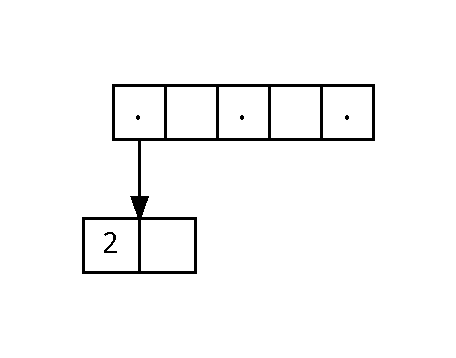
\includegraphics[scale=0.4]{./dot/A1_1-01.pdf}\\
  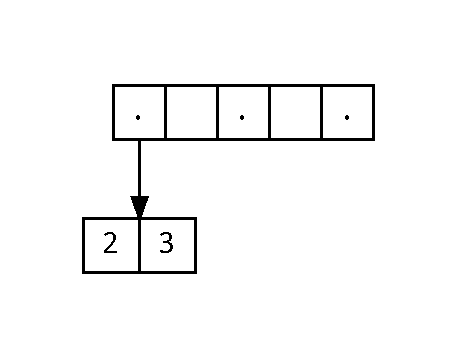
\includegraphics[scale=0.4]{./dot/A1_1-02.pdf}\\
  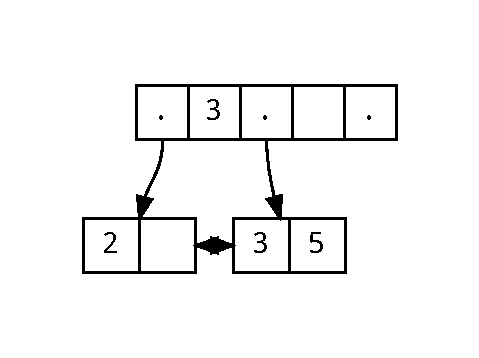
\includegraphics[scale=0.4]{./dot/A1_1-03.pdf}\\
  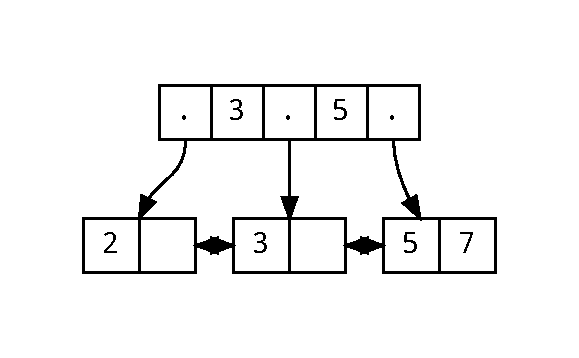
\includegraphics[scale=0.4]{./dot/A1_1-04.pdf}\\
  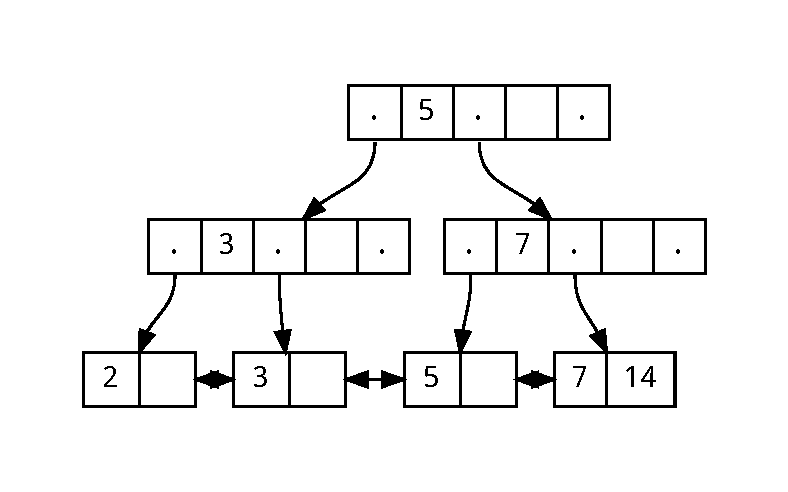
\includegraphics[scale=0.4]{./dot/A1_1-05.pdf}\\
  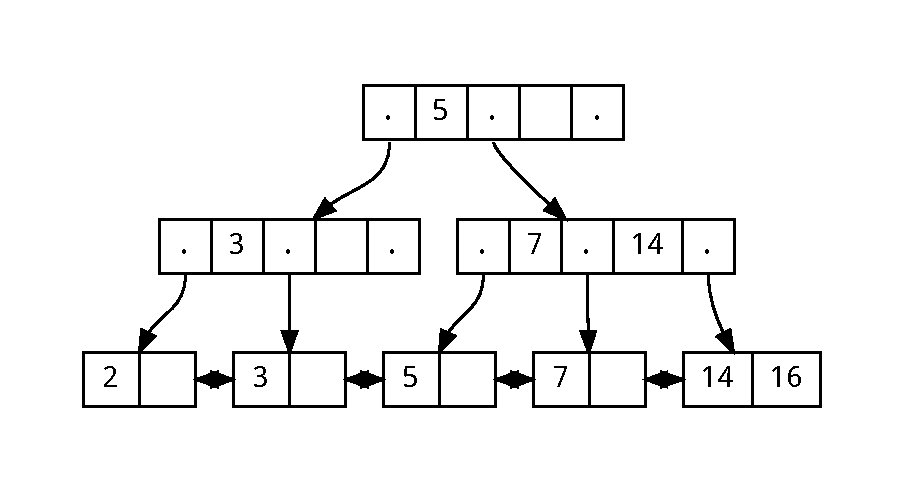
\includegraphics[scale=0.4]{./dot/A1_1-06.pdf}\\
  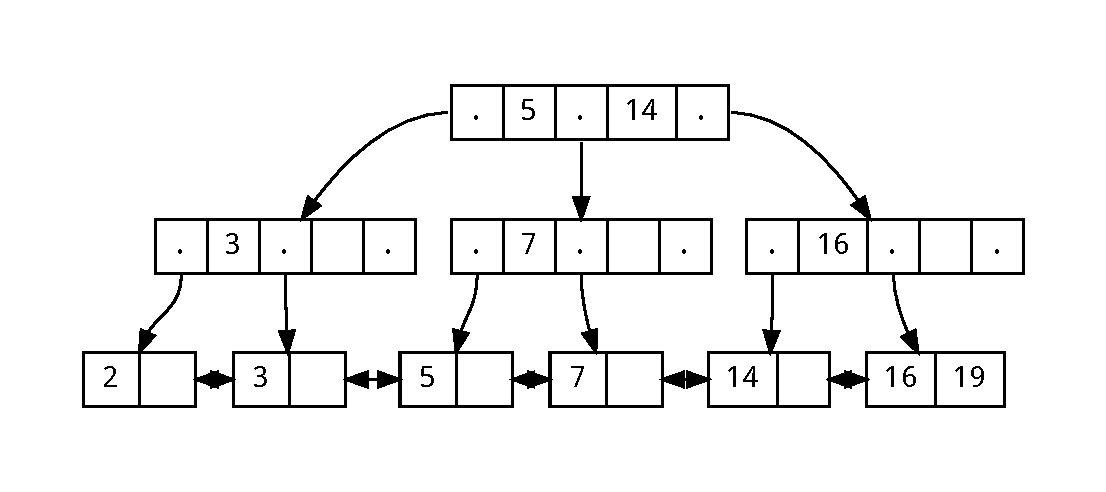
\includegraphics[scale=0.4]{./dot/A1_1-07.pdf}\\
  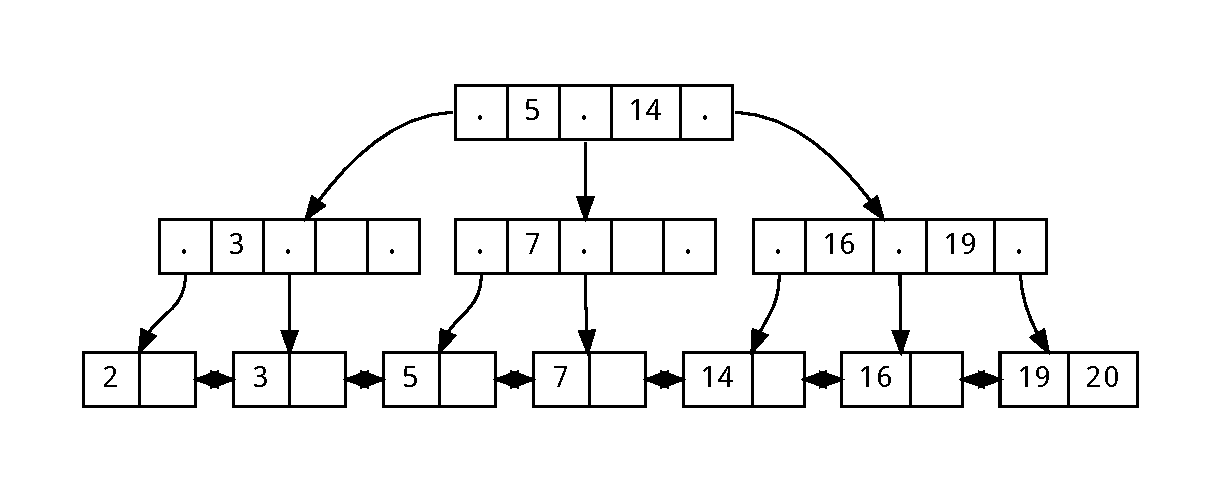
\includegraphics[scale=0.4]{./dot/A1_1-08.pdf}\\
  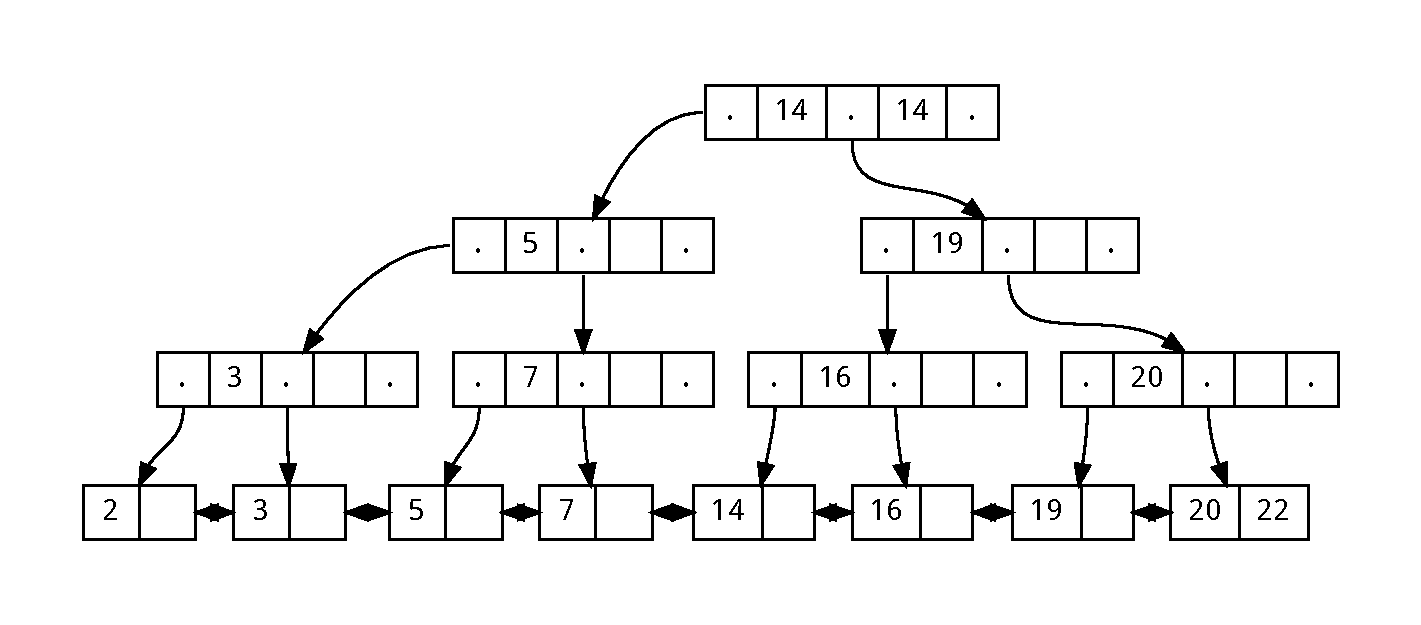
\includegraphics[scale=0.4]{./dot/A1_1-09.pdf}\\
  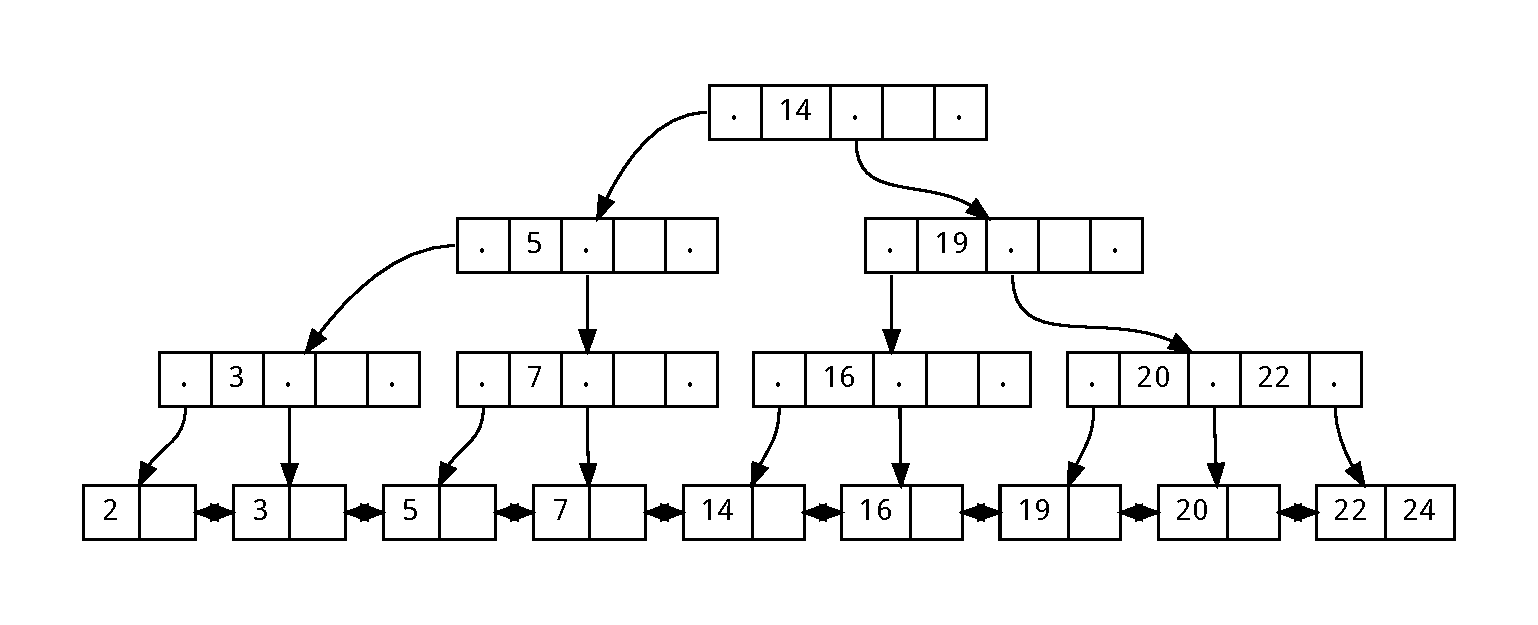
\includegraphics[scale=0.4]{./dot/A1_1-10.pdf}\\
  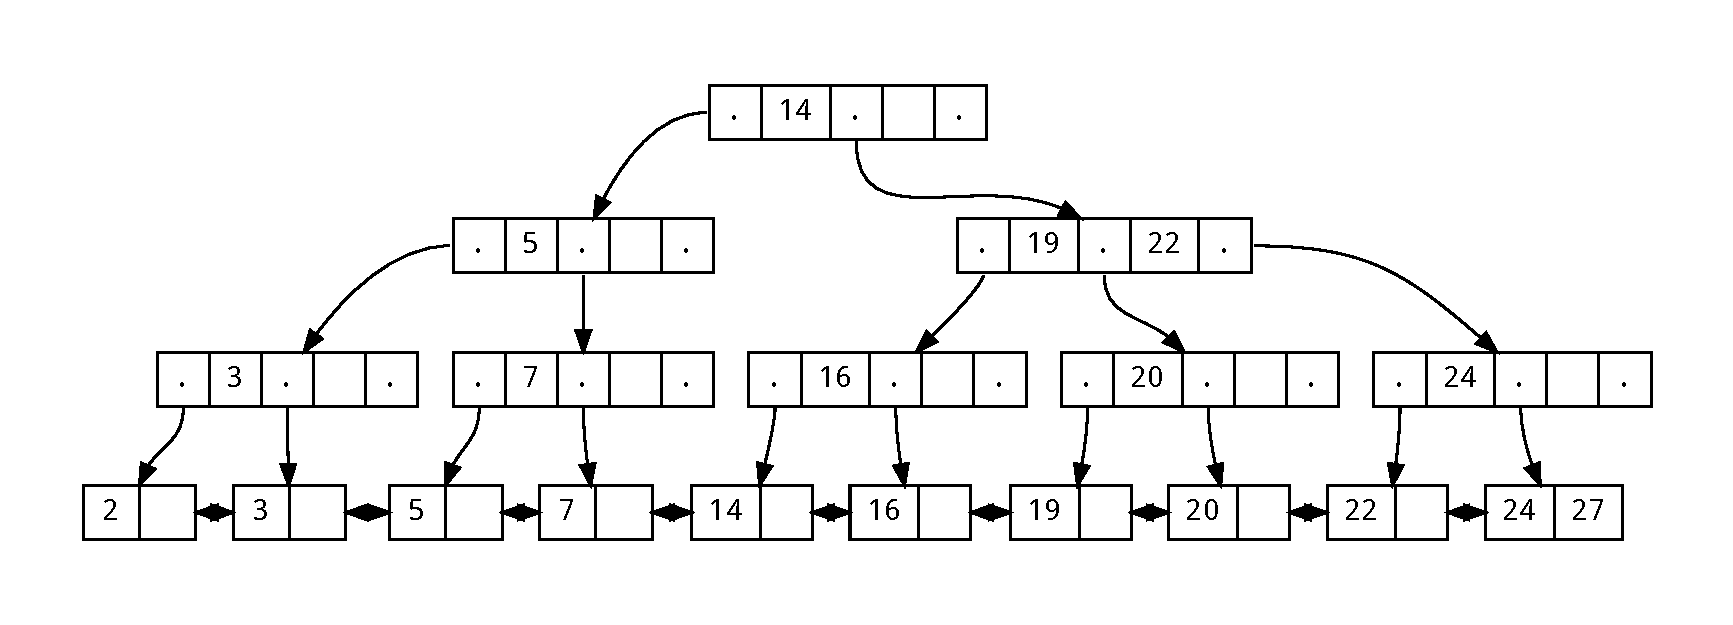
\includegraphics[scale=0.4]{./dot/A1_1-11.pdf}\\
  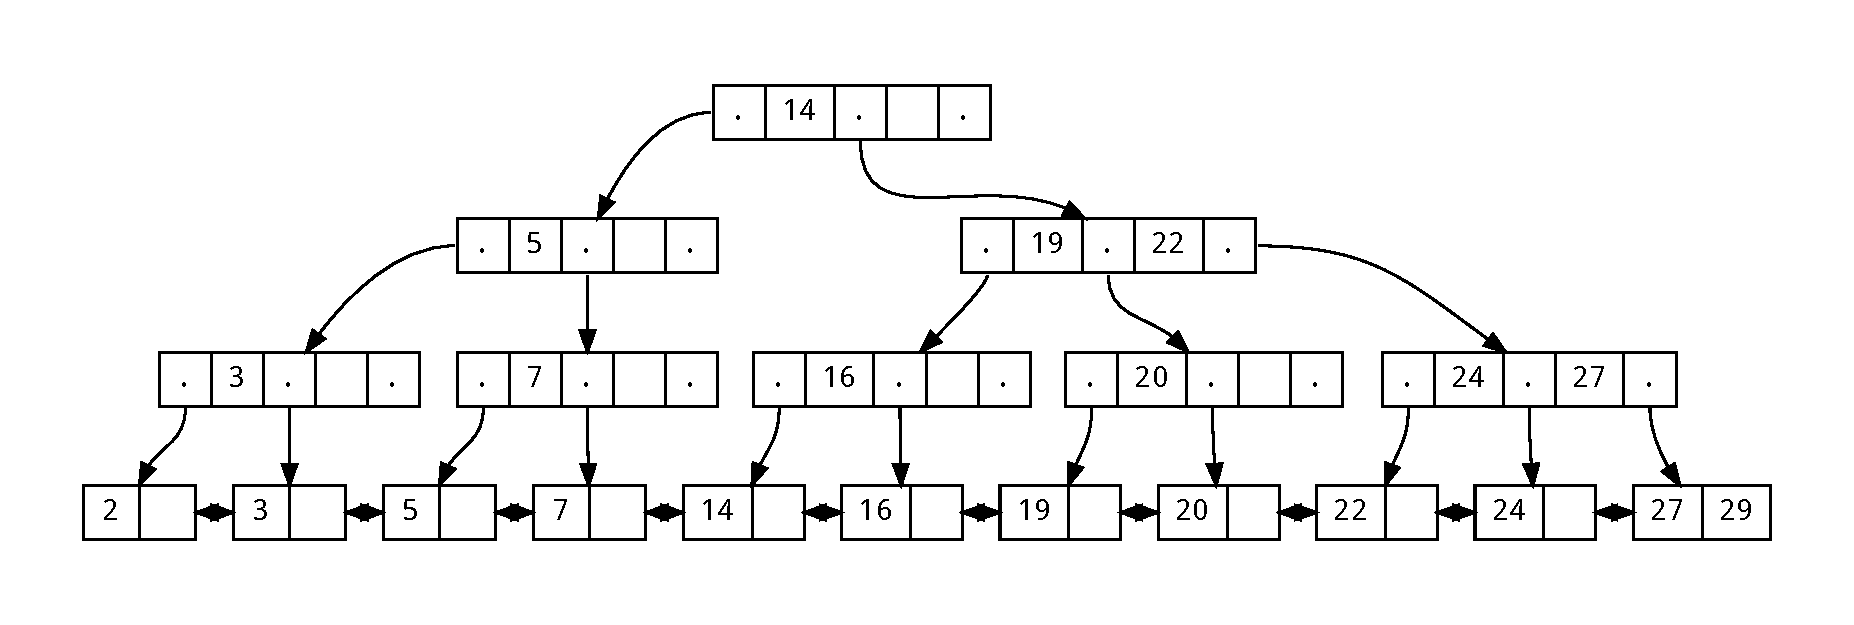
\includegraphics[scale=0.4]{./dot/A1_1-12.pdf}\\
  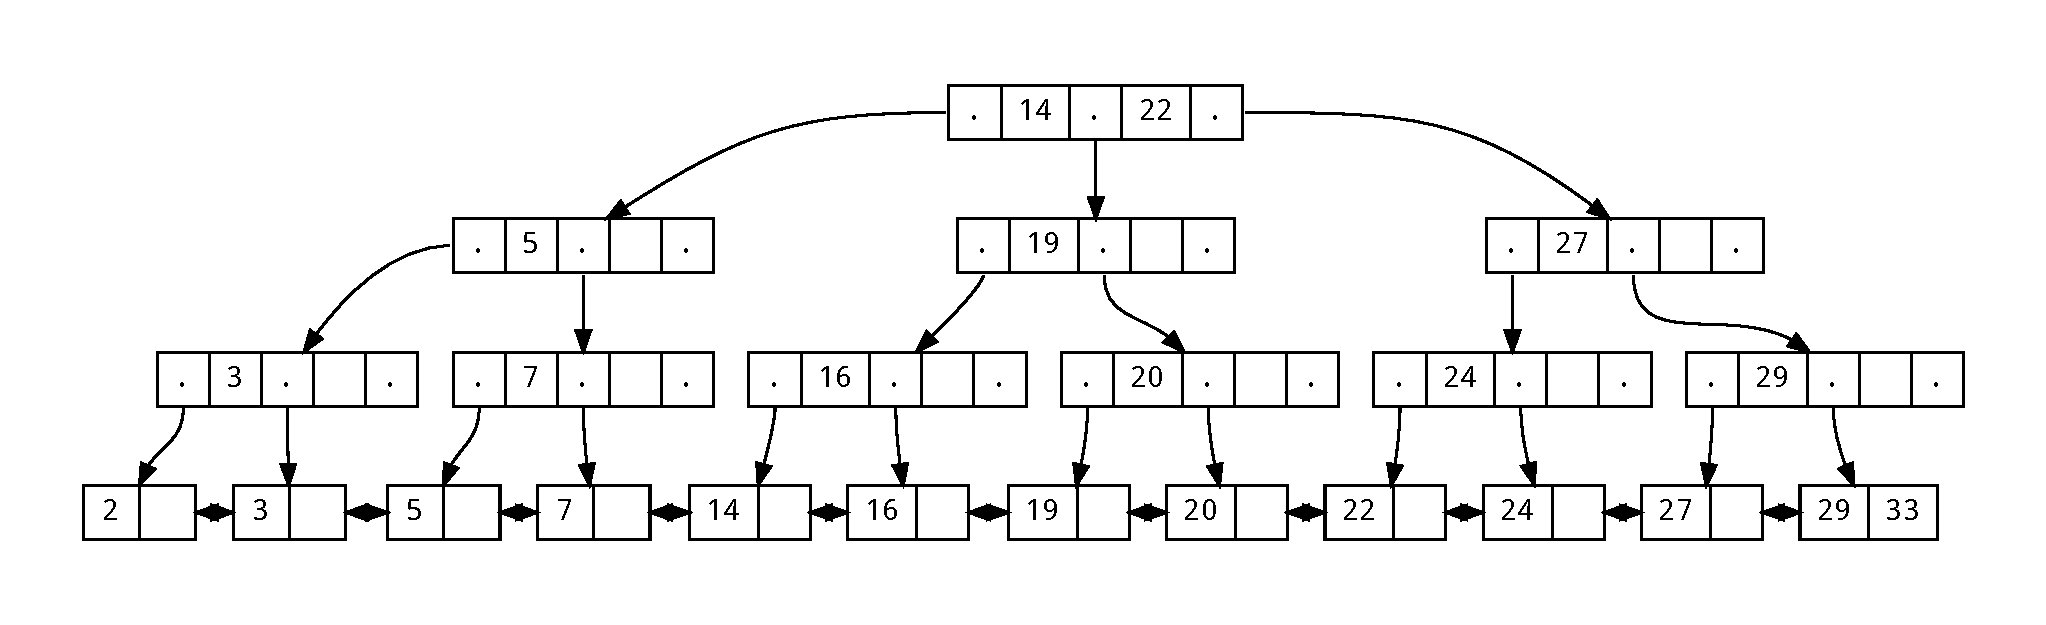
\includegraphics[scale=0.4]{./dot/A1_1-13.pdf}\\
  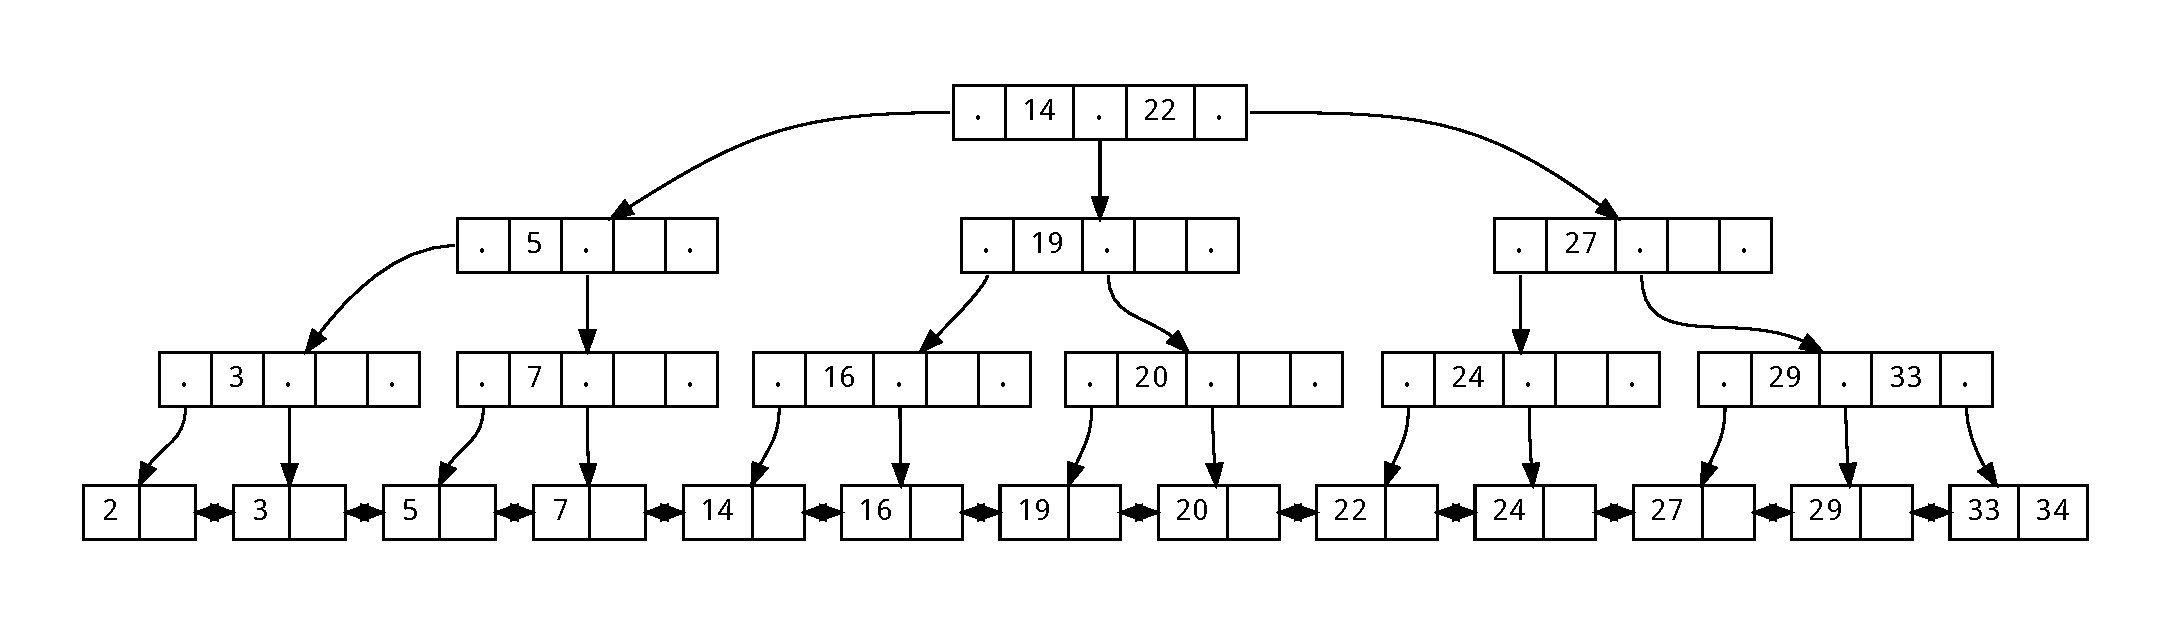
\includegraphics[scale=0.4]{./dot/A1_1-14.pdf}\\
  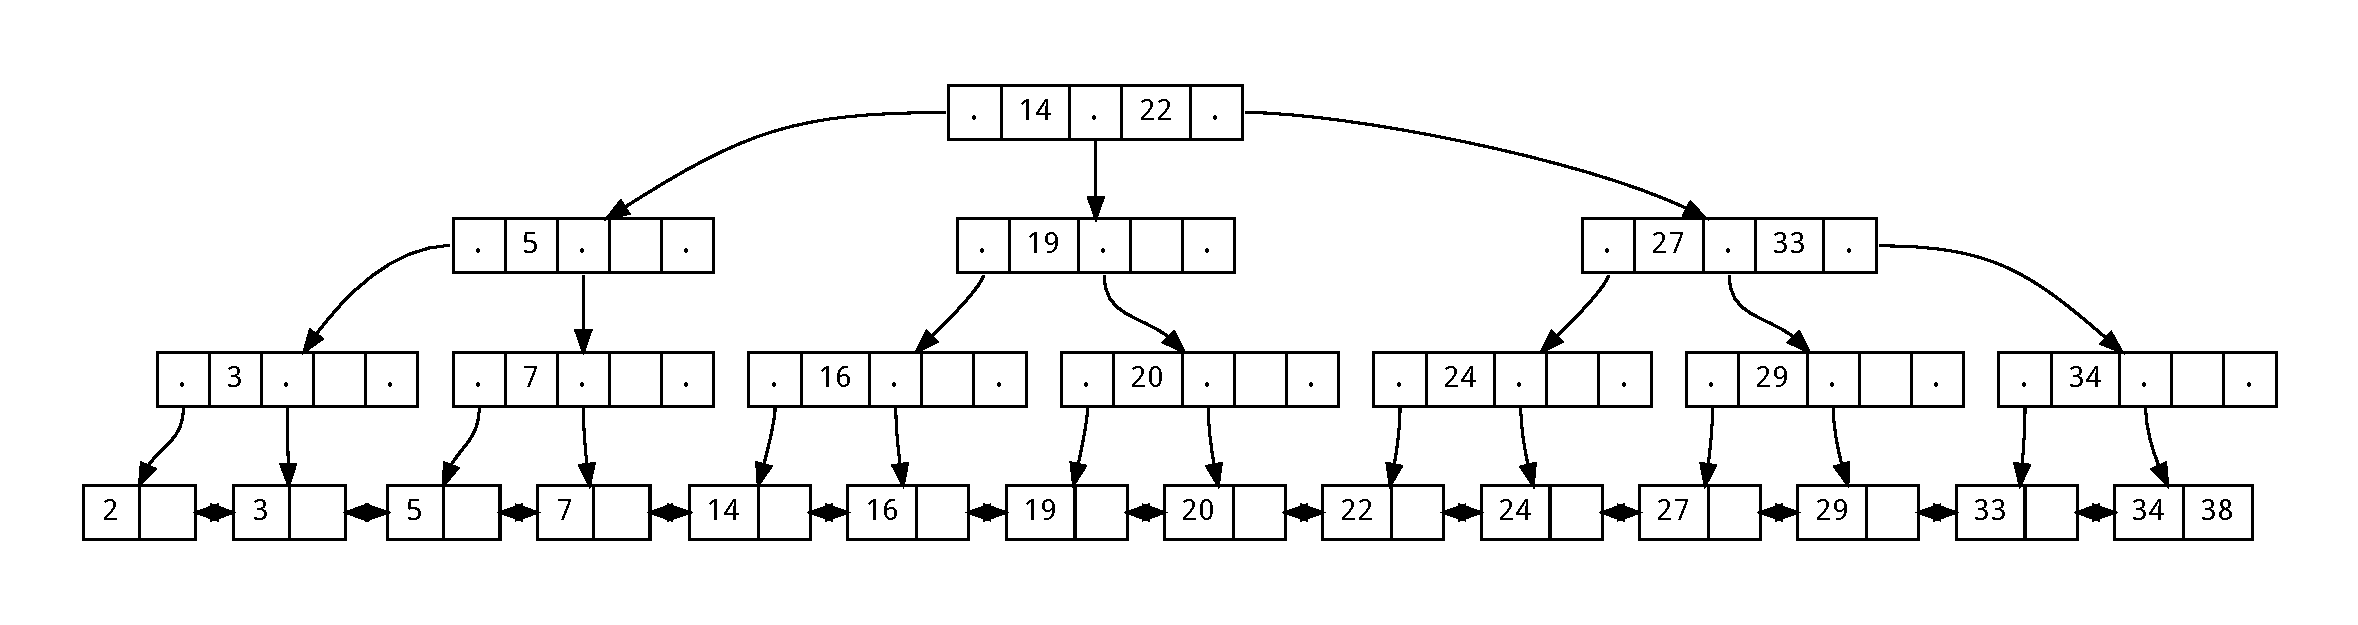
\includegraphics[scale=0.4]{./dot/A1_1-15.pdf}\\
  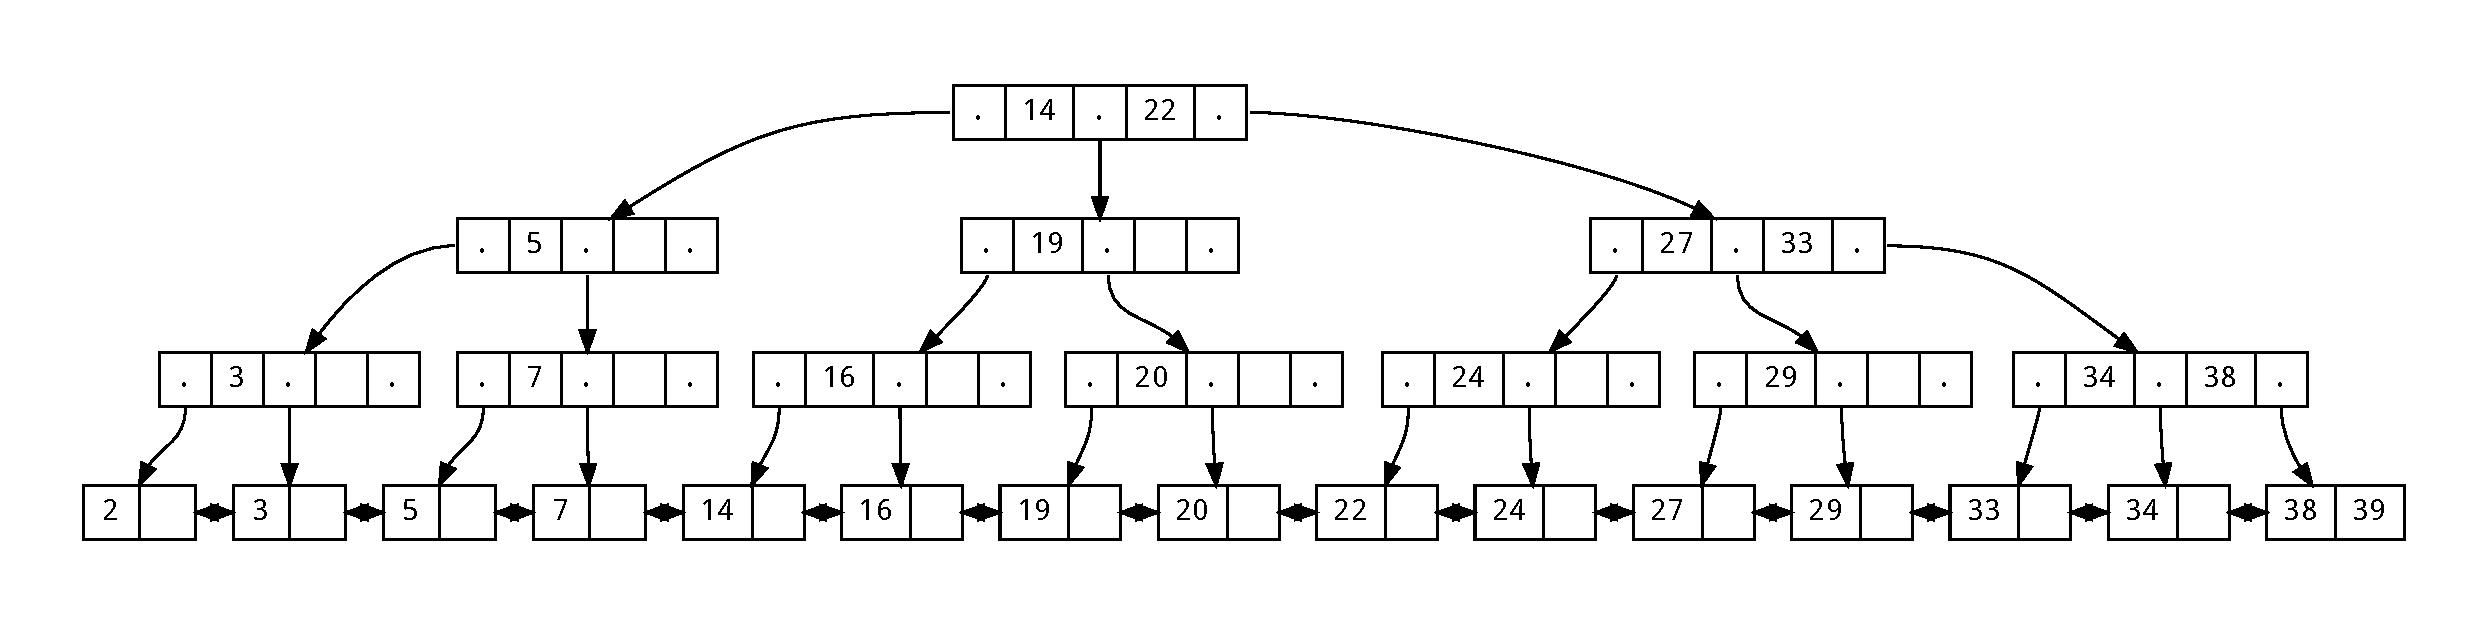
\includegraphics[scale=0.4]{./dot/A1_1-16.pdf}
\subExEnd{}
%
\newpage 
%
\exercise{}
\subExBegin{1{.}}
  \item \emph{Benennen Sie alle Knoten $(I_j\text{ bzw. }L_k)$, die betrachtet werden müssen, um die folgende Anfrage zu beantworten: "Suchen Sie alle Tupel mit einem Schlüssel größer als 38."}\\
  Besucht werden müssen: $I_1, I_2, L_2, L_3, L_4, L_5$
  \item \emph{Fügen Sie ein Tupel mit Schlüssel $109$ in den Baum ein. Geben Sie den resultierenden Baum an.}\\
  Der nicht gezeichnete Teilbaum bleibt unverändert.\\
  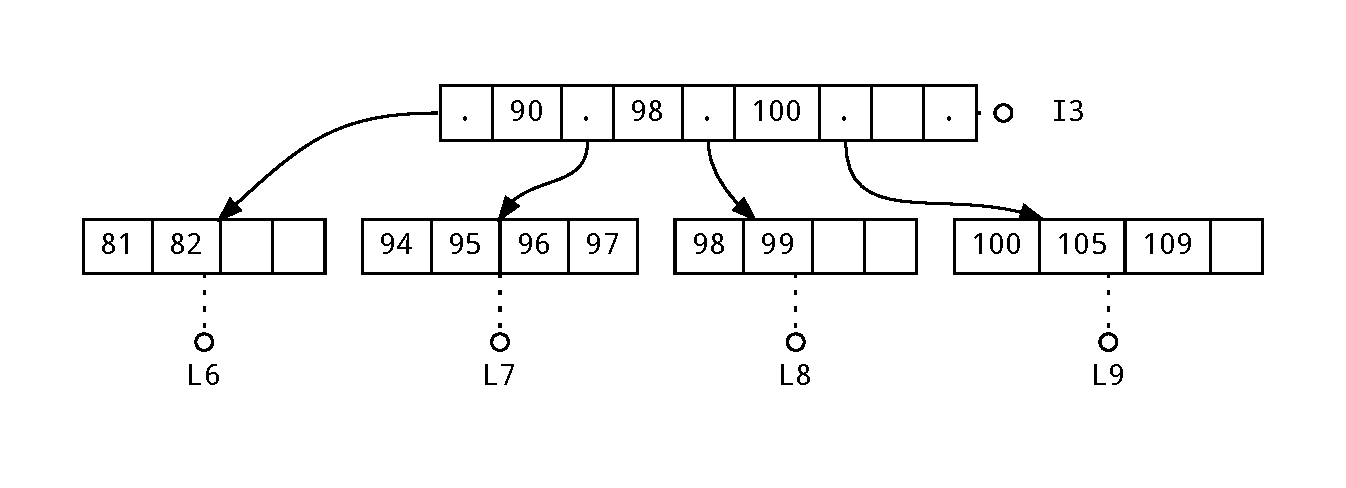
\includegraphics[scale=0.4]{./dot/A2_2.pdf}
  \item \emph{Finden Sie einen Schlüsselwert, der beim Eintragen in den Originalbaum eine Erhöhung des Baumes bewirkt.}\\
  Mögliche Schlusselwerte sind:\\$k \in \set{N}: (\text{Überlauf \code{L4}}) \lor \text{Überlauf \code{L5}}) \Leftrightarrow (50 \leq k < 65 \lor 65 \leq k < 80)$, da mit einem Überlauf von \code{L4} oder \code{L5} nachfolgend \code{I2} und damit \code{I1} überlaufen.
  \item \emph{Beachten Sie, dass die Teilbäume $A, B, C$ in Abbildung 2 nicht vollständig spezifiziert wurden. Was können Sie dennoch über den Inhalt und die Struktur dieser Teilbäume schließen.}\\
  Die Bereiche der untergeordneten Schlüssel, wie folgt:
  \begin{description}
    \item[$A:$] $k < 10$
    \item[$B:$] $10 < k < 20$
    \item[$C:$] $20 < k < 30$
  \end{description}
  \item \emph{Stellen Sie sich vor, der Index auf Abbildung 2 sei ein ISAM Index. Bestimmen Sie die minimale Anzahl an Einträgen, um eine Kette von drei \emph{overflow pages} zu generieren.}\\
  Der Baum bietet nur mit Schüsselwerten $k \in \set{N}: 106 \leq k$ die Möglichkeit eine \emph{Kette} von drei (oder mehr) \code{overflow pages} zu generieren. Die minimale Anzahl an Schlüsselwerten, sodass $3$ Kettenglieder entstehen entspricht $9$ Schlüsseln, da mit dem $9.$ Schlüssel die dritte \code{overflow page} angelegt wird.
\subExEnd{}
%
\newpage 
%
\exercise{}
\subExBegin{1{.}}
  \item \emph{Identifizieren Sie $5$ Blattknoten-Einträge, so dass das Einfügen der Einträge in der von Ihnen zu wählenden Reihenfolge und das Löschen in der umgekehrten Reihenfolge $(\text{z.B.}, \code{insert } a, \code{insert } b, \code{delete } b, \code{delete } a)$ in einem anderen Baum, als in Abbildung 1 resultiert.}\\
  $13, 15, 21, 25, 40$\\
  Nach \code{insert}:\\
  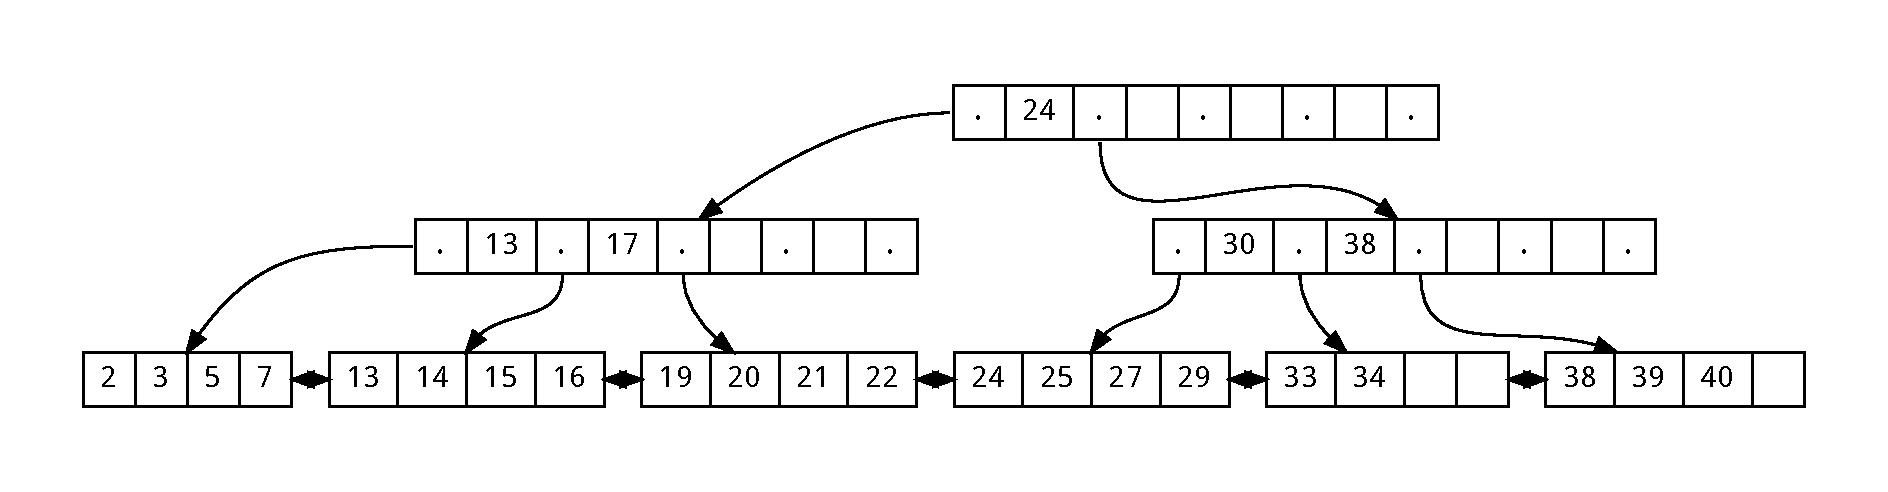
\includegraphics[scale=0.4]{./dot/A3_1-1.pdf}\\
  Nach \code{delete}:\\
  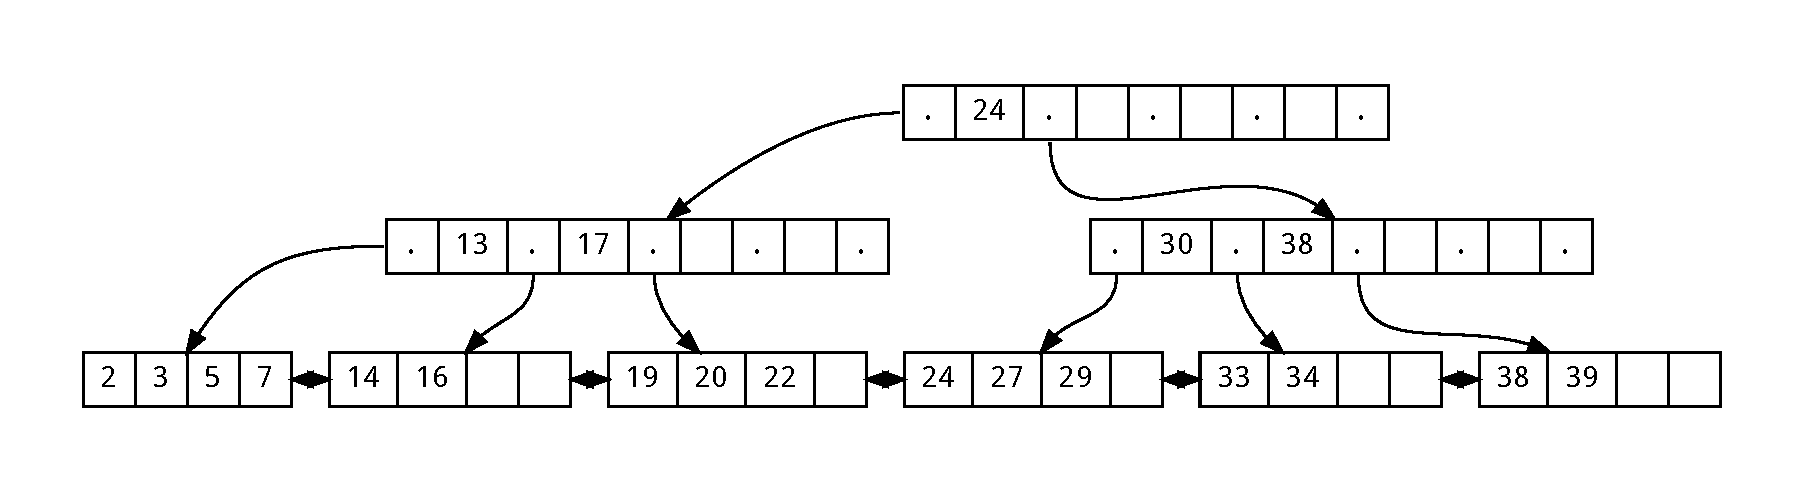
\includegraphics[scale=0.4]{./dot/A3_1-2.pdf}
  \item \emph{Identifizieren Sie $5$ Blattknoten-Einträge, so dass das Einfügen der Einträge in der von Ihnen zu wählenden Reihenfolge und das Löschen in der umgekehrten Reihenfolge $(\text{z.B.}, \code{insert } a, \code{insert } b, \code{delete } b, \code{delete } a)$ wieder im Originalbaum in Abbildung 1 resultiert.}\\
  $1, 4, 13, 15, 21$\\
  Nach \code{insert}:\\
  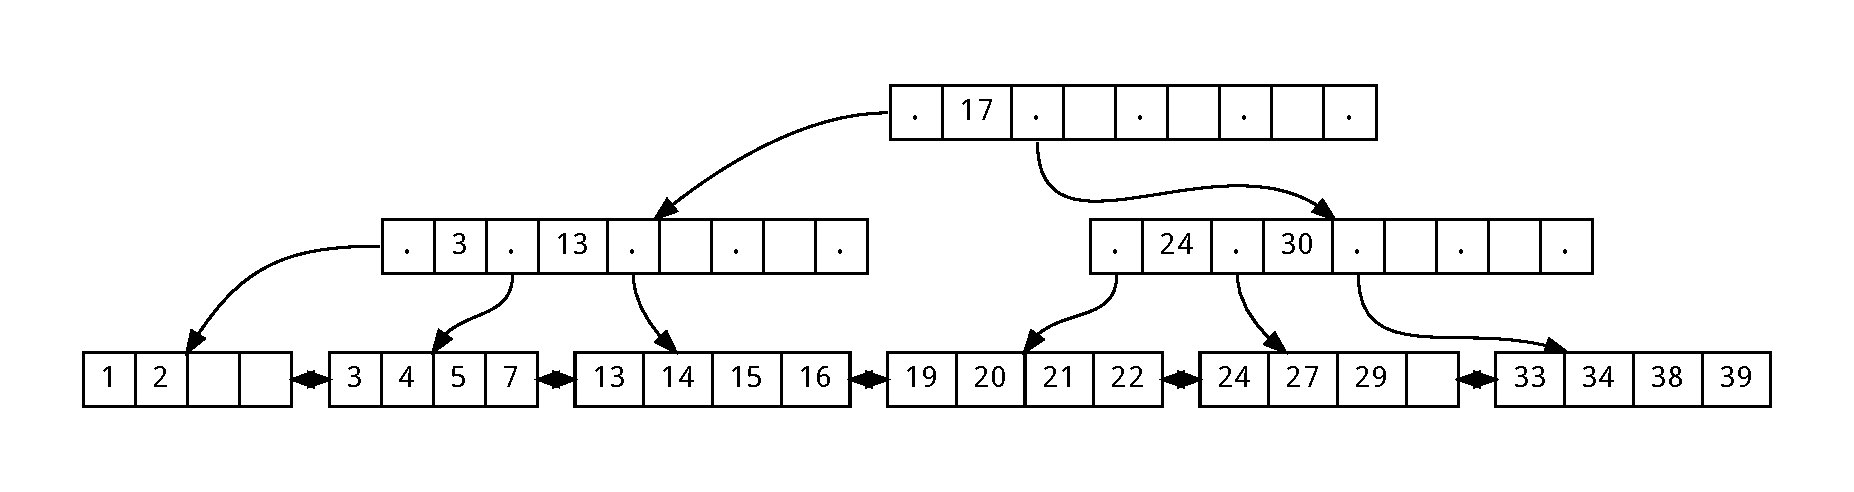
\includegraphics[scale=0.4]{./dot/A3_2-1.pdf}\\
  Vor letztem \code{delete}:\\
  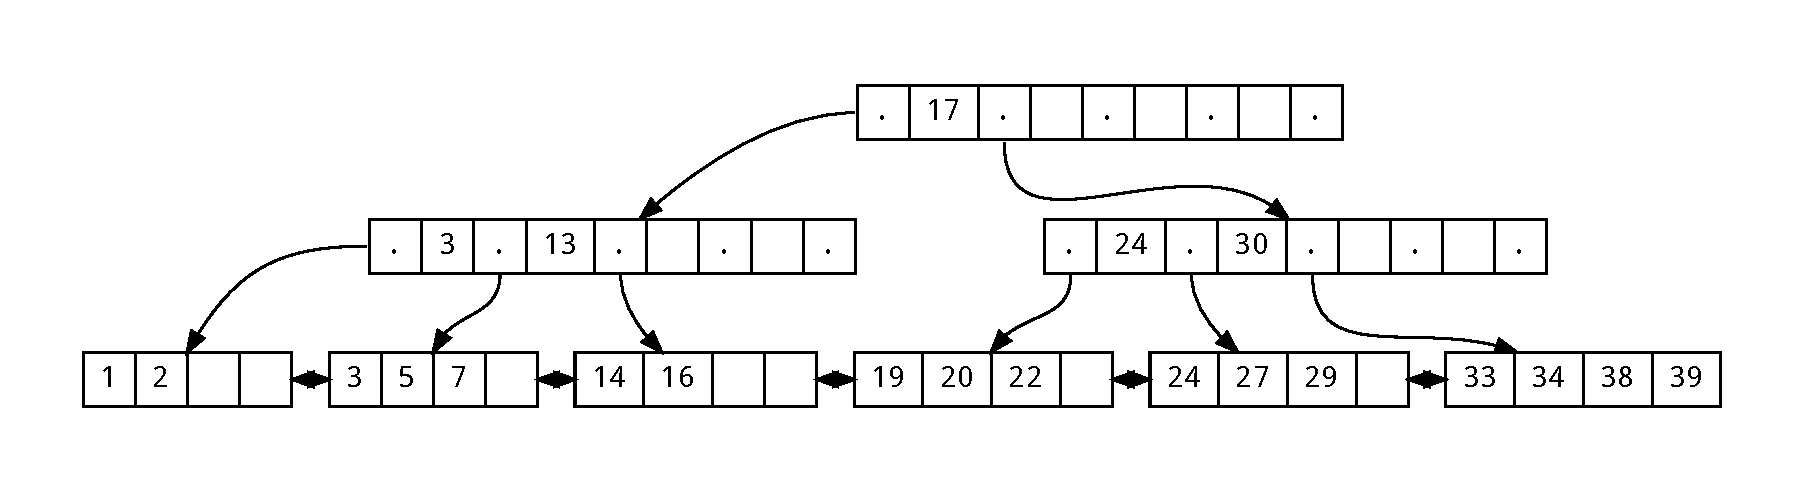
\includegraphics[scale=0.4]{./dot/A3_2-2.pdf}\\
  Die durch den \code{delete(1)} hervorgerufenen Unterläufe führen zu merges, die den ursp. Graph hervorbringen.
  
\subExEnd{}

\end{document}